\documentclass[11pt]{beamer}
\usetheme{Warsaw}
\usepackage[utf8]{inputenc}
\usepackage[spanish]{babel}
\usepackage{amsmath,amsthm,amssymb} %modos matemáticos y  simbolos
\usepackage{latexsym,amsfonts} %simbolos matematicos
\usepackage{graphicx}
\usepackage{physics} %Simbolos fisicos
\usepackage{array} %mejores formatos de tabla
\usepackage{tabulary}
\usepackage{multirow} %ocupar varias filas en una tabla
\usepackage{fancybox} %recuadros talegas
\usepackage{float} %ubicar graficas
\usepackage{color}
\usepackage{comment}
\usepackage{stackrel}
\usepackage{calligra}
\usepackage{lipsum} % texto de relleno
\usepackage{cite}
\author{Diego Sarceño \\ \footnotesize{201900109}}
\title{Parcial 1 \\ \footnotesize{Materia Condensada 2}}
%\setbeamercovered{transparent} 
%\setbeamertemplate{navigation symbols}{} 
%\logo{} 
%\institute{} 
\date{\today} 
%\subject{} 
\begin{document}

\begin{frame}
\titlepage
\end{frame}

%\begin{frame}
%\tableofcontents
%\end{frame}

\frame{
	\frametitle{Capítulo 9 Problema 6 Enunciado}
	\begin{enumerate}[a)]
		\item Encuentre una expresión para la energía de unión de un electrón en una dimensión en un pozo cuadrado simple de profundidad $U_o$ y ancho $a$. (Asuma que la solución es simétrica respecto del punto medio del pozo)
		\item Encuentre un resultado numérico para la energía de unión en términos de $U_o$ para el caso especial de $\abs{U_o} = \flatfrac{2\hbar ^2}{ma^2}$ y comparelo con el límite apropiado de la figura $20$. En este límite de pozos muy separados el ancho de banda llega a cero, por lo que la energía de $k = 0$ es la misma que la energía para cualquier otra $k$ en la banda de energía más baja. Otras bandas estan formadas de los estados excitados del pozo, en este límite.
	\end{enumerate}
}



\frame{
	\frametitle{Capítulo 9 Problema 6 Enunciado}
	\begin{figure}[H]
		\centering
		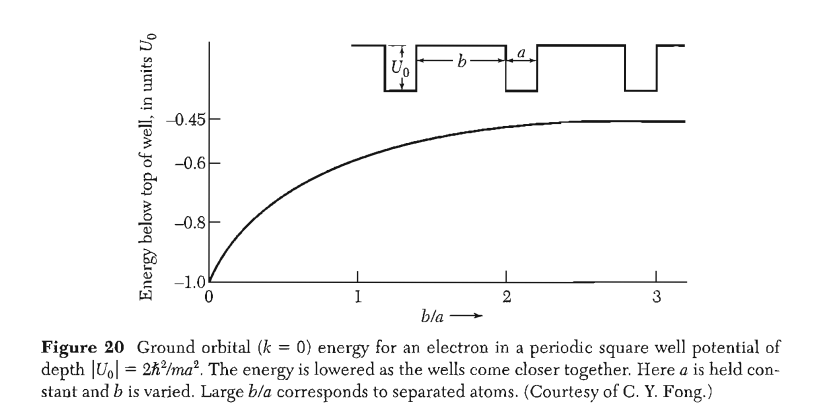
\includegraphics[scale=0.3]{./img/fig20.png}
		\caption{Figura $20$, $"$Introduction to solid state physics$"$ - Wiley, Kittel.}
		\label{kittel20}
	\end{figure}
}




\frame{
	\frametitle{Solución}
	\only<1>{ \vspace{1.5cm}
	\begin{figure}[H]
		\centering
		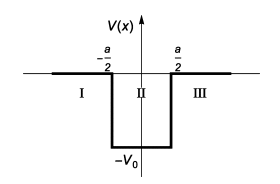
\includegraphics[scale=0.5]{./img/well.png}
		\caption{Pozo de potencial.}
		\label{well}
	\end{figure}	
	}
	\onslide<2->{Para la región del pozo, se tiene la ecuación de Schrodinger
		$$ \qty(-\frac{\hbar}{2m} \dv[2]{x} - U_o) \psi = E\psi $$}
	\onslide<3->{Cuya solución es $\psi _{II} = B\cos{kx}$.}
	\onslide<4->{Mientras que para la región anterior al pozo (que es la otra región de interés) la ecuación y su solución es:}
	\onslide<5->{$$ -\frac{\hbar}{2m} \dv[2]{x} \psi = E\psi \qquad \Rightarrow \qquad \psi _{I} = Ae^{\kappa x}. $$}
	\onslide<6->{Donde
	$$ \kappa = \sqrt{-\frac{2mE}{\hbar ^2}}, \quad k = \sqrt{\frac{2m(E + U_o)}{\hbar ^2}}. $$}
}

\frame{
	\frametitle{Solución}
	\onslide<1->{Por lo que
		$$ \boxed{E = -\frac{\hbar ^2 \kappa ^2}{2m}, \quad E = \frac{\hbar ^2 k^2}{2m} - U_o .} $$}
	\onslide<2->{Además, en el límite de la energía de unión ($x = -a/2$), las funciones propias y sus primeras derivadas deben ser continuas en las discontinuidades del potencial, es decir:}
	\onslide<3->{$$ \psi _{I} (-a/2) = \psi _{II} (-a/2), \quad \psi ' _{I} (-a/2) = \psi ' _{II} (-a/2). $$}	
	\onslide<4->{Dividiendo estas dos ecuaciones se tiene la siguiente relación:}
	\onslide<5->{
	\begin{equation}
		\boxed{ \kappa = k\tan{\frac{ka}{2}} .} \label{tan}
	\end{equation}}
}




\frame{
	\frametitle{Solución}
	Es lógico pensar que las energías deber ser iguales bajo la relación \eqref{tan}, sin embargo, es necesaria una implementación numérica\footnote{Una implementación posible es la proporcionada por \href{http://hyperphysics.phy-astr.gsu.edu/hbase/quantum/pfbox.html}{Hyperphysics}} para resolver esto. Por lo que se dará por hecho y tomando la figura \ref{kittel20} la energía que cumple con lo solicitada es $\boxed{E = -0.45}$, ya que hace que hace que los pozos estén lo suficientemente separados para que la energía $k = 0$ sea la misma que cualquier otra $k$ en la banda de energía más baja.

}







\frame{
	\frametitle{Capítulo 9 Problema 7 Enunciado}
	\begin{enumerate}[a)]
		\item Calcule el periodo $\Delta (1/B)$ esperado para el potasio en el modelo de electrón libre.
		\item Cuál es el área en el espacio real de la orbita externa, para $B = 10kG = 1T$? El mismo periodo se aplica a oscilaciones en la resistividad eléctrica, conocida como el efecto Shubnikow-de Haas.
	\end{enumerate}
}




\frame{
	\frametitle{Solución}
	\onslide<1->{\textit{(a)} Tomando la periodicidad en el efecto Haas$-$Van Alphen}
	\onslide<2->{$$ \Delta \qty(\frac{1}{B}) = \frac{2\pi e}{\hbar c S}. $$}
	\onslide<3->{En donde $S = 4\pi k_F ^2$, este $k_F$ lo encontramos en la tabla $1$ capítulo $6$. \\}
	\only<4>{
		\begin{figure}[H]
			\centering
			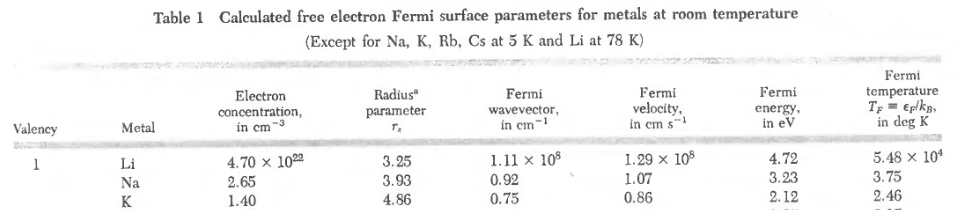
\includegraphics[scale=0.3]{./img/potaxio.png}
		\end{figure}			
	}
	\onslide<5->{Con lo que, luego de valuar en sistema CGS: $\Delta (1/B) = 1.35\times 10^{-9} G^{-1}$.}

		
}


\frame{
	\frametitle{Solución}
		\onslide<1->{\textit{(b)} Tenemos la relación entre la velocidad y la frecuencia angular: $\omega _c R = v_F$ con $\omega _c = eB/mc$. \\}
		\onslide<2->{Además, por la cuantización del momentum: $p_F = mv_F = \hbar k_F$, se reemplaza en lo anterior y se tiene}
		\onslide<3->{$$ R = \frac{\hbar k_F c}{eB}, $$}
		\onslide<4->{$$\text{Area} = \pi R^2 = 4.94\times 10^{-4}cm ^2$$}
}

\frame{
	\centering
	\vspace{1cm}
	GRACIAS POR SU ATENCIÓN $<3$
}














\end{document}